\subsection{调试过程}

\qquad 智能风扇控制系统的调试工作按照模块化的思路进行,采用分模块测试、功能验证、集成调试的步骤,确保每个功能模块的正确性和系统整体的稳定性。

\subsubsection{系统初始化调试}

\qquad 系统初始化是整个项目的基础,包括STM32微控制器时钟配置、GPIO初始化、外设配置等关键环节。

\textbf{调试内容:}
\begin{itemize}
    \vspace{-6pt}
  \item 验证系统时钟频率设置(168MHz)是否正确
    \vspace{-6pt}
  \item 检查各外设模块初始化函数的执行状态
    \vspace{-6pt}
  \item 确认GPIO引脚配置与硬件连接的一致性
    \vspace{-6pt}
  \item 测试系统启动后的基本响应能力
\end{itemize}

\textbf{调试方法:}通过LED指示灯闪烁和串口输出信息验证系统成功启动,观察各初始化函数的返回值。

% 预留图片位置
\begin{figure}[H]
  \centering
  \includegraphics[width=0.45\textwidth]{../figures/CleanShot 2025-06-11 at 11.48.35@2x.png}
  \caption{系统初始化调试过程}
  \label{fig:system_init_debug}
\end{figure}

\subsubsection{LCD显示功能调试}

\qquad LCD显示是人机交互的重要组成部分,需要验证文字显示、中文支持、居中对齐等功能。

\textbf{调试内容:}
\begin{itemize}
    \vspace{-6pt}
  \item 验证LCD初始化是否成功,屏幕是否正常点亮
    \vspace{-6pt}
  \item 测试中英文混合字符的正确显示
    \vspace{-6pt}
  \item 检验文字居中对齐算法的准确性
    \vspace{-6pt}
  \item 确认实时数据更新显示的正确性
\end{itemize}

\textbf{调试方法:}逐步显示不同内容,验证\texttt{get\_centered\_x()}函数和\texttt{update\_display()}函数的功能。

\subsubsection{按键控制功能调试}

\qquad 按键是用户操作的主要接口,需要验证按键检测、中断响应、防抖处理等功能。

\textbf{调试内容:}
\begin{itemize}
    \vspace{-6pt}
  \item 测试K1-K4四个按键的中断触发功能
    \vspace{-6pt}
  \item 验证按键防抖延时(50ms)的有效性
    \vspace{-6pt}
  \item 检查按键功能映射的正确性
    \vspace{-6pt}
  \item 确认按键响应的实时性和准确性
\end{itemize}

\textbf{调试方法:}通过串口输出按键值,结合蜂鸣器确认音验证按键功能,测试连续按键和长按的处理。

\subsubsection{温湿度检测功能调试}

\qquad HTU21D传感器是环境监测的核心器件,需要验证I2C通信、数据准确性、更新频率等。

\textbf{调试内容:}
\begin{itemize}
    \vspace{-6pt}
  \item 验证HTU21D传感器的I2C通信是否正常
    \vspace{-6pt}
  \item 测试温度和湿度数据的读取准确性
    \vspace{-6pt}
  \item 检查数据格式化显示(温度2位小数,湿度1位小数)
    \vspace{-6pt}
  \item 确认传感器响应速度和数据稳定性
\end{itemize}

\textbf{调试方法:}通过串口实时输出温湿度数据,与标准测量设备对比验证精度,测试不同环境条件下的响应。

% 预留图片位置
\begin{figure}[H]
  \centering
  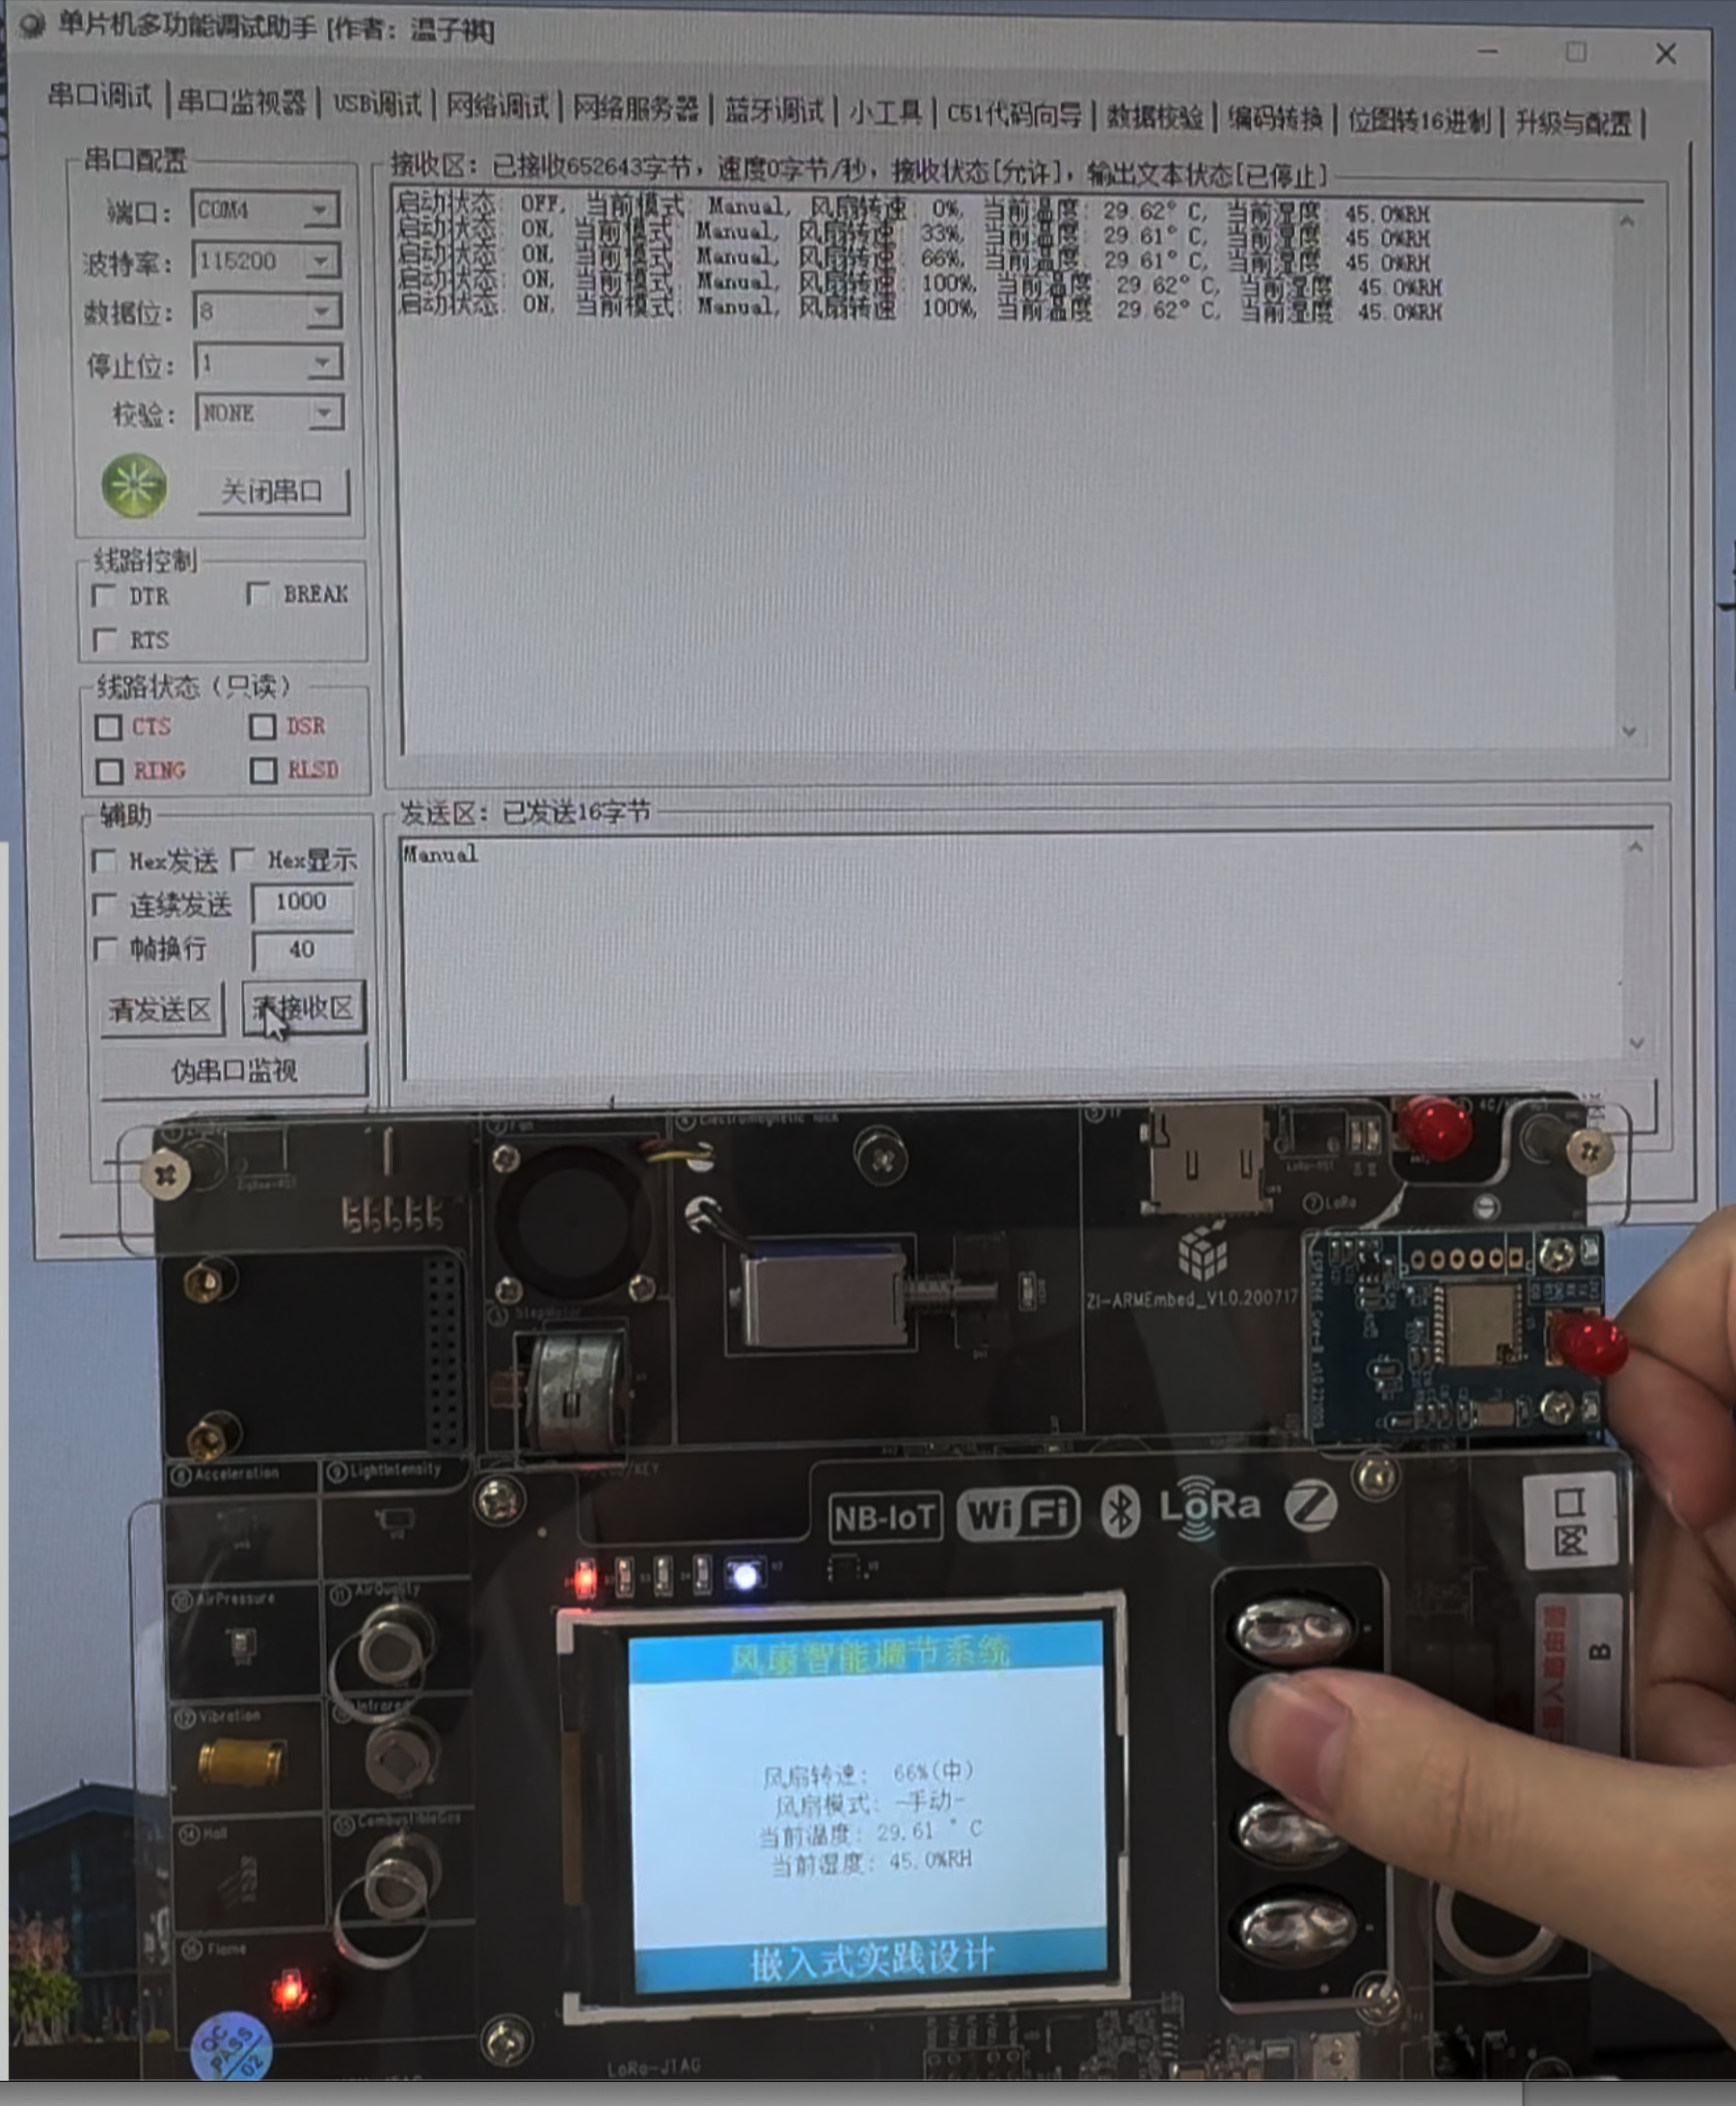
\includegraphics[width=0.45\textwidth]{../figures/CleanShot 2025-06-11 at 11.50.13@2x.png}
  \caption{温湿度检测功能调试结果}
  \label{fig:htu21d_debug}
\end{figure}

\subsubsection{风扇PWM控制功能调试}

\qquad 风扇控制是系统的核心执行功能,需要验证PWM输出、档位切换、转速精度等。

\textbf{调试内容:}
\begin{itemize}
    \vspace{-6pt}
  \item 验证PWM信号输出频率(50kHz)和占空比准确性
    \vspace{-6pt}
  \item 测试0档(0\%)、1档(33\%)、2档(66\%)、3档(100\%)四个档位
    \vspace{-6pt}
  \item 检查档位切换的平滑性和响应速度
    \vspace{-6pt}
  \item 确认风扇运行的稳定性和噪音水平
\end{itemize}

\textbf{调试方法:}使用示波器测量PWM信号,观察风扇转速变化,测试长时间运行稳定性。

\subsubsection{RGB LED状态指示功能调试}

\qquad RGB LED提供直观的系统状态指示,需要验证颜色控制、状态映射等功能。

\textbf{调试内容:}
\begin{itemize}
    \vspace{-6pt}
  \item 测试RGB LED的基本颜色显示功能
    \vspace{-6pt}
  \item 验证不同风扇档位对应的颜色指示
    \vspace{-6pt}
  \item 检查状态变化时LED的响应速度
    \vspace{-6pt}
  \item 确认LED亮度和颜色的视觉效果
\end{itemize}

\textbf{调试方法:}手动切换风扇档位,观察RGB LED颜色变化,验证状态指示的准确性和直观性。

% 预留图片位置
\begin{figure}[H]
  \centering
  \begin{subfigure}{0.45\textwidth}
    \centering
    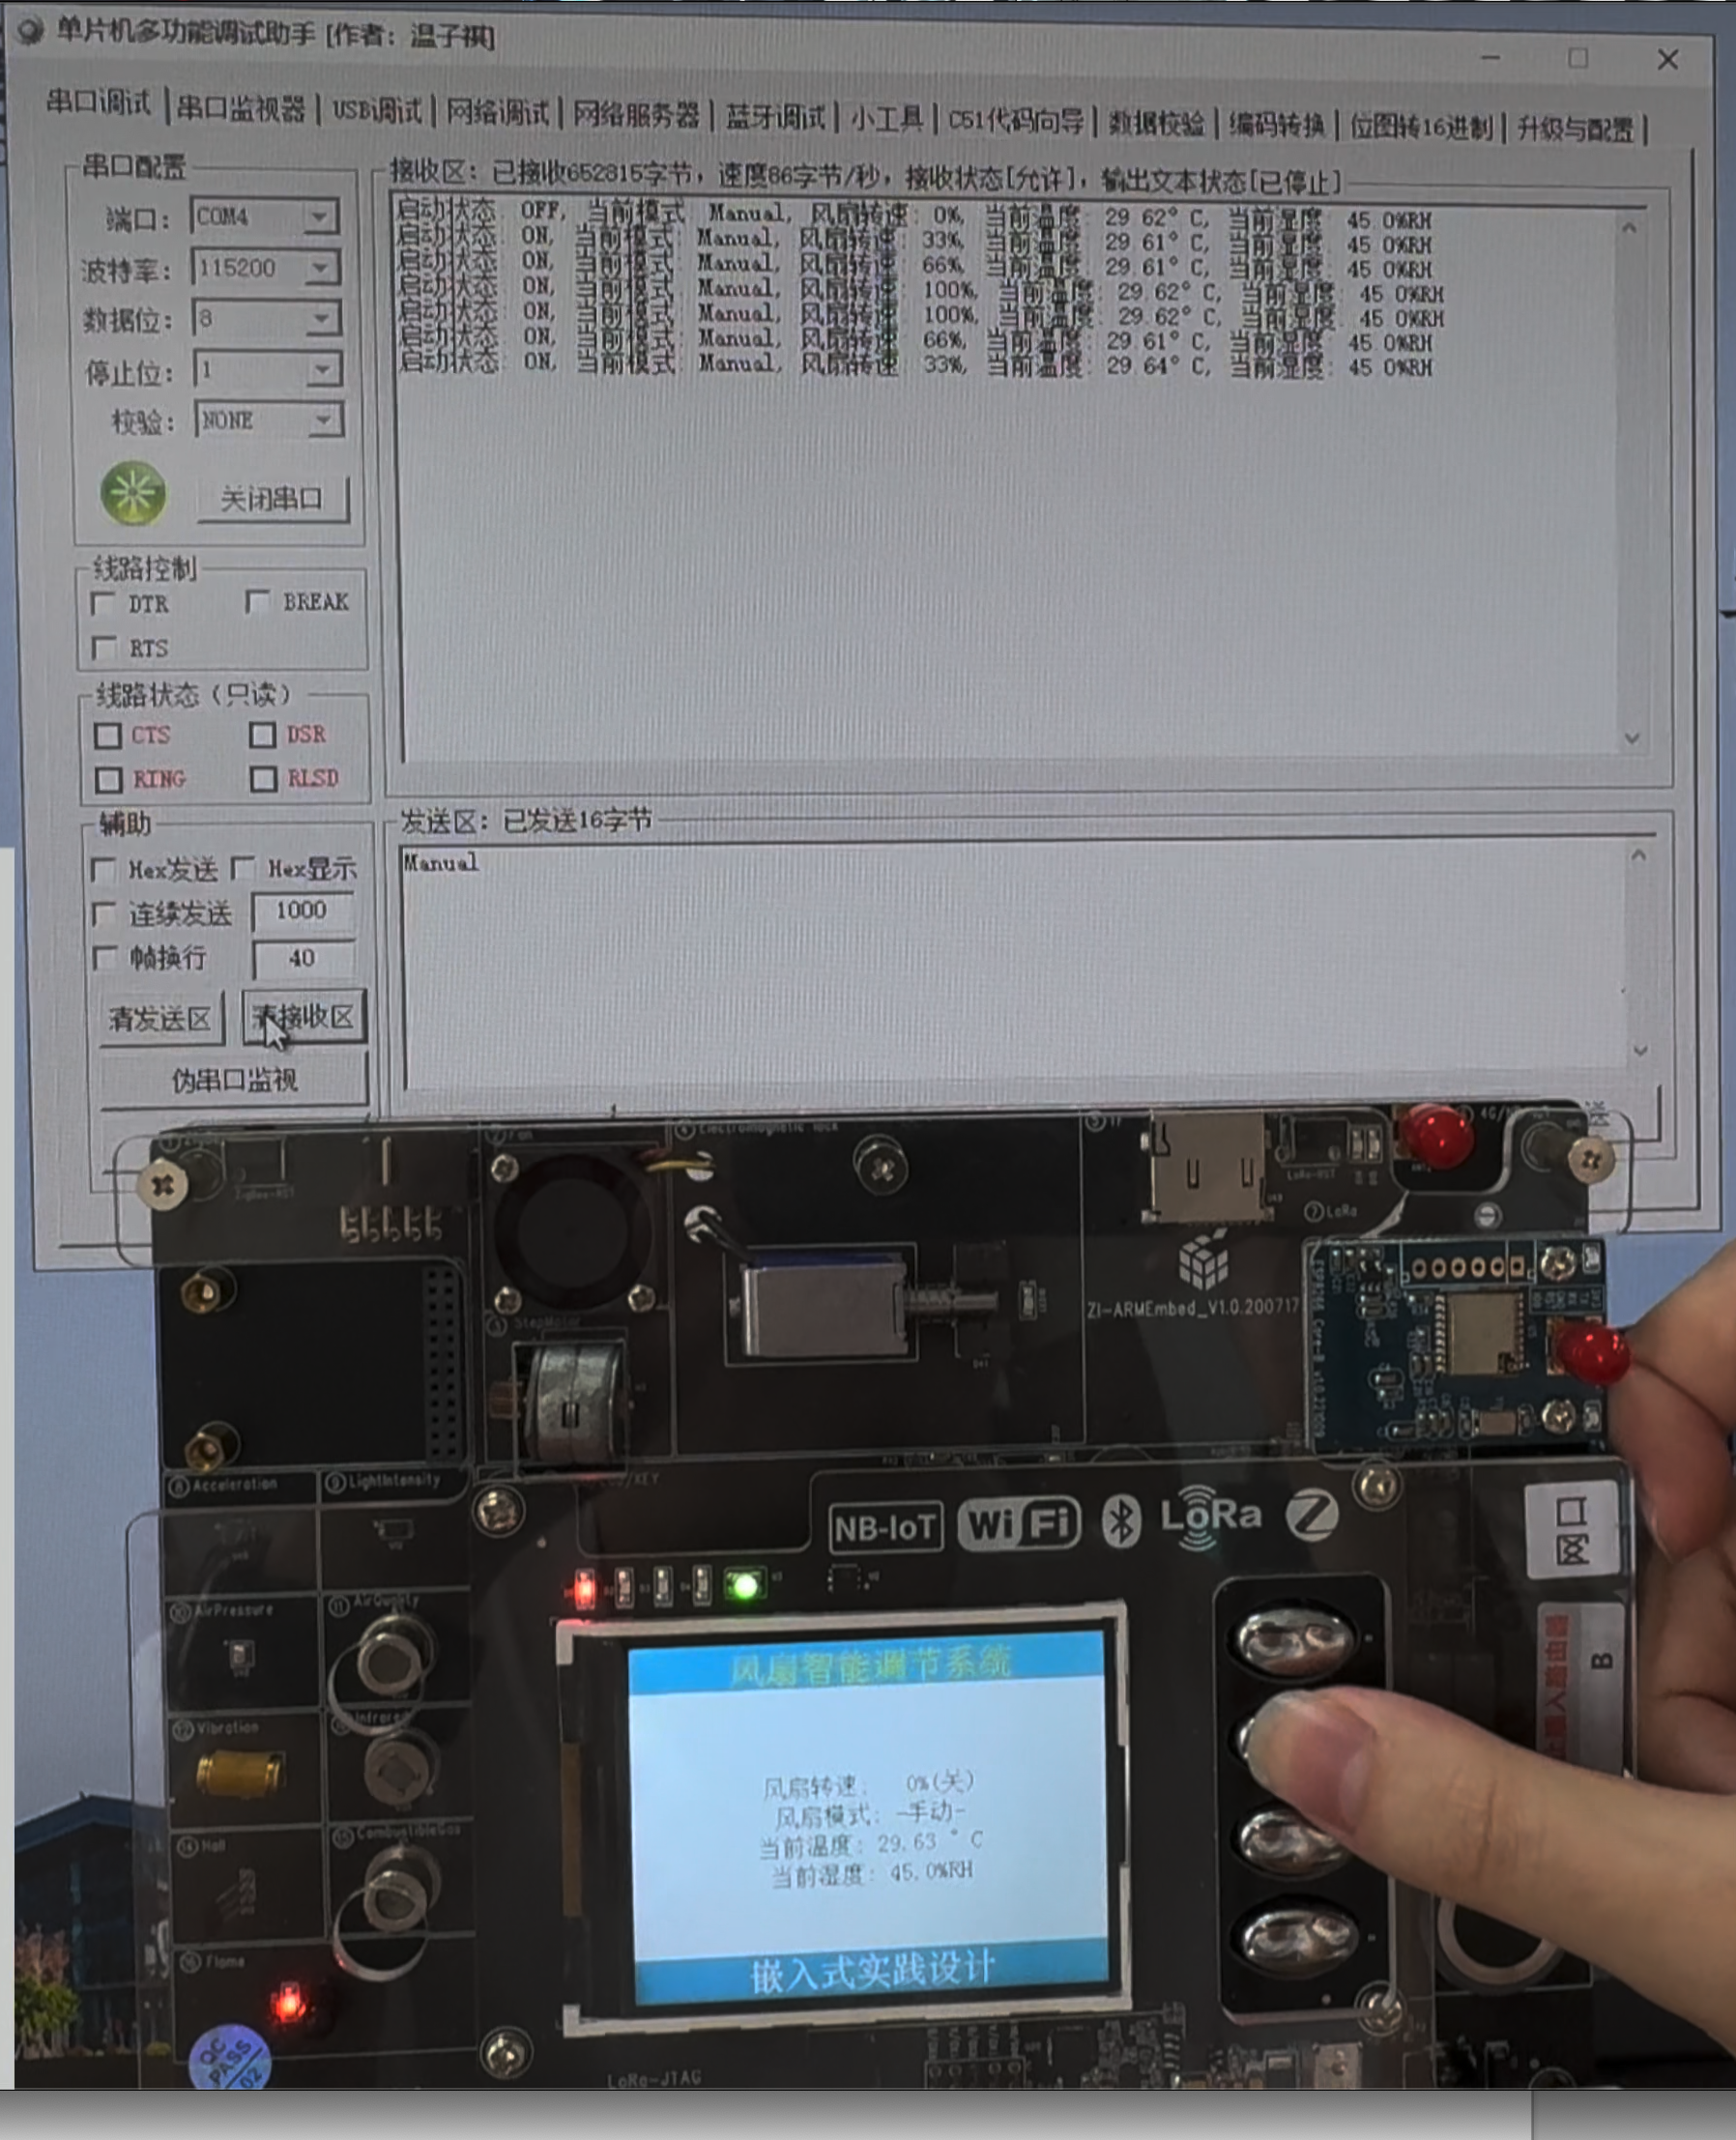
\includegraphics[width=\textwidth]{../figures/CleanShot 2025-06-11 at 11.53.10@2x.png}
    \caption{风扇关闭状态}
  \end{subfigure}
  \hfill
  \begin{subfigure}{0.45\textwidth}
    \centering
    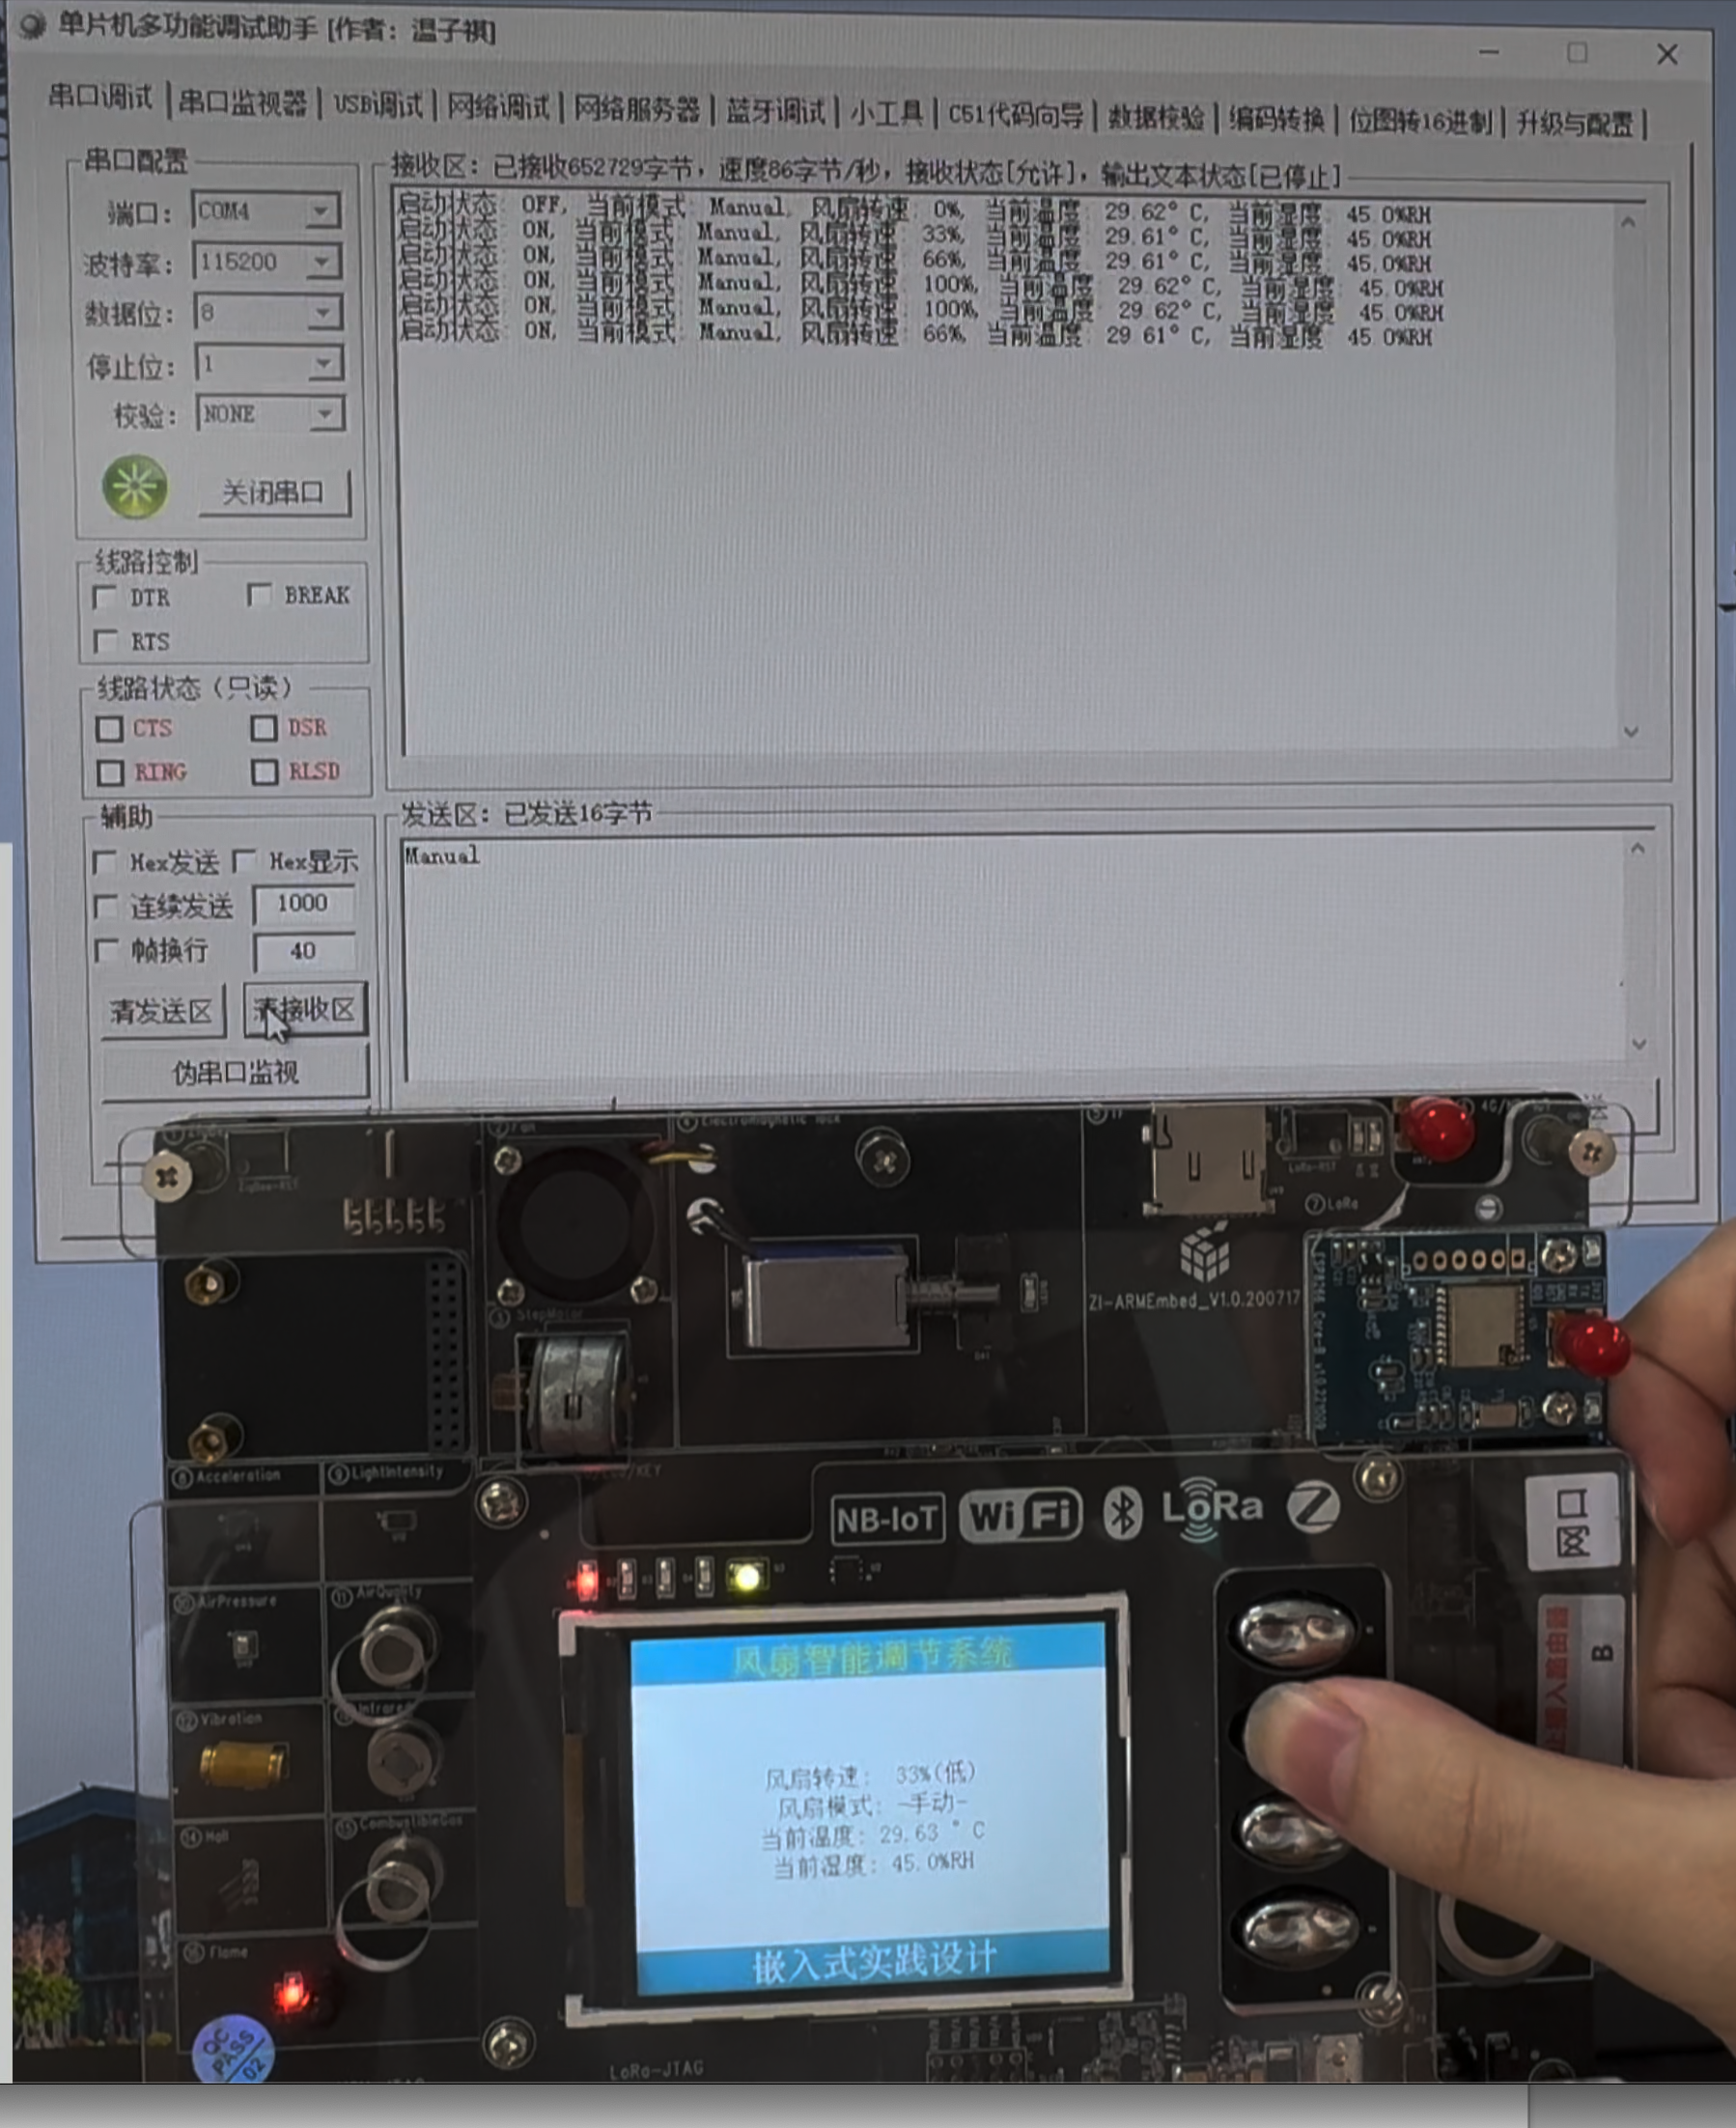
\includegraphics[width=\textwidth]{../figures/CleanShot 2025-06-11 at 11.52.57@2x.png}
    \caption{风扇转速33\%状态}
  \end{subfigure}

  \vspace{1pt}

  \centering
  \begin{subfigure}{0.45\textwidth}
    \centering
    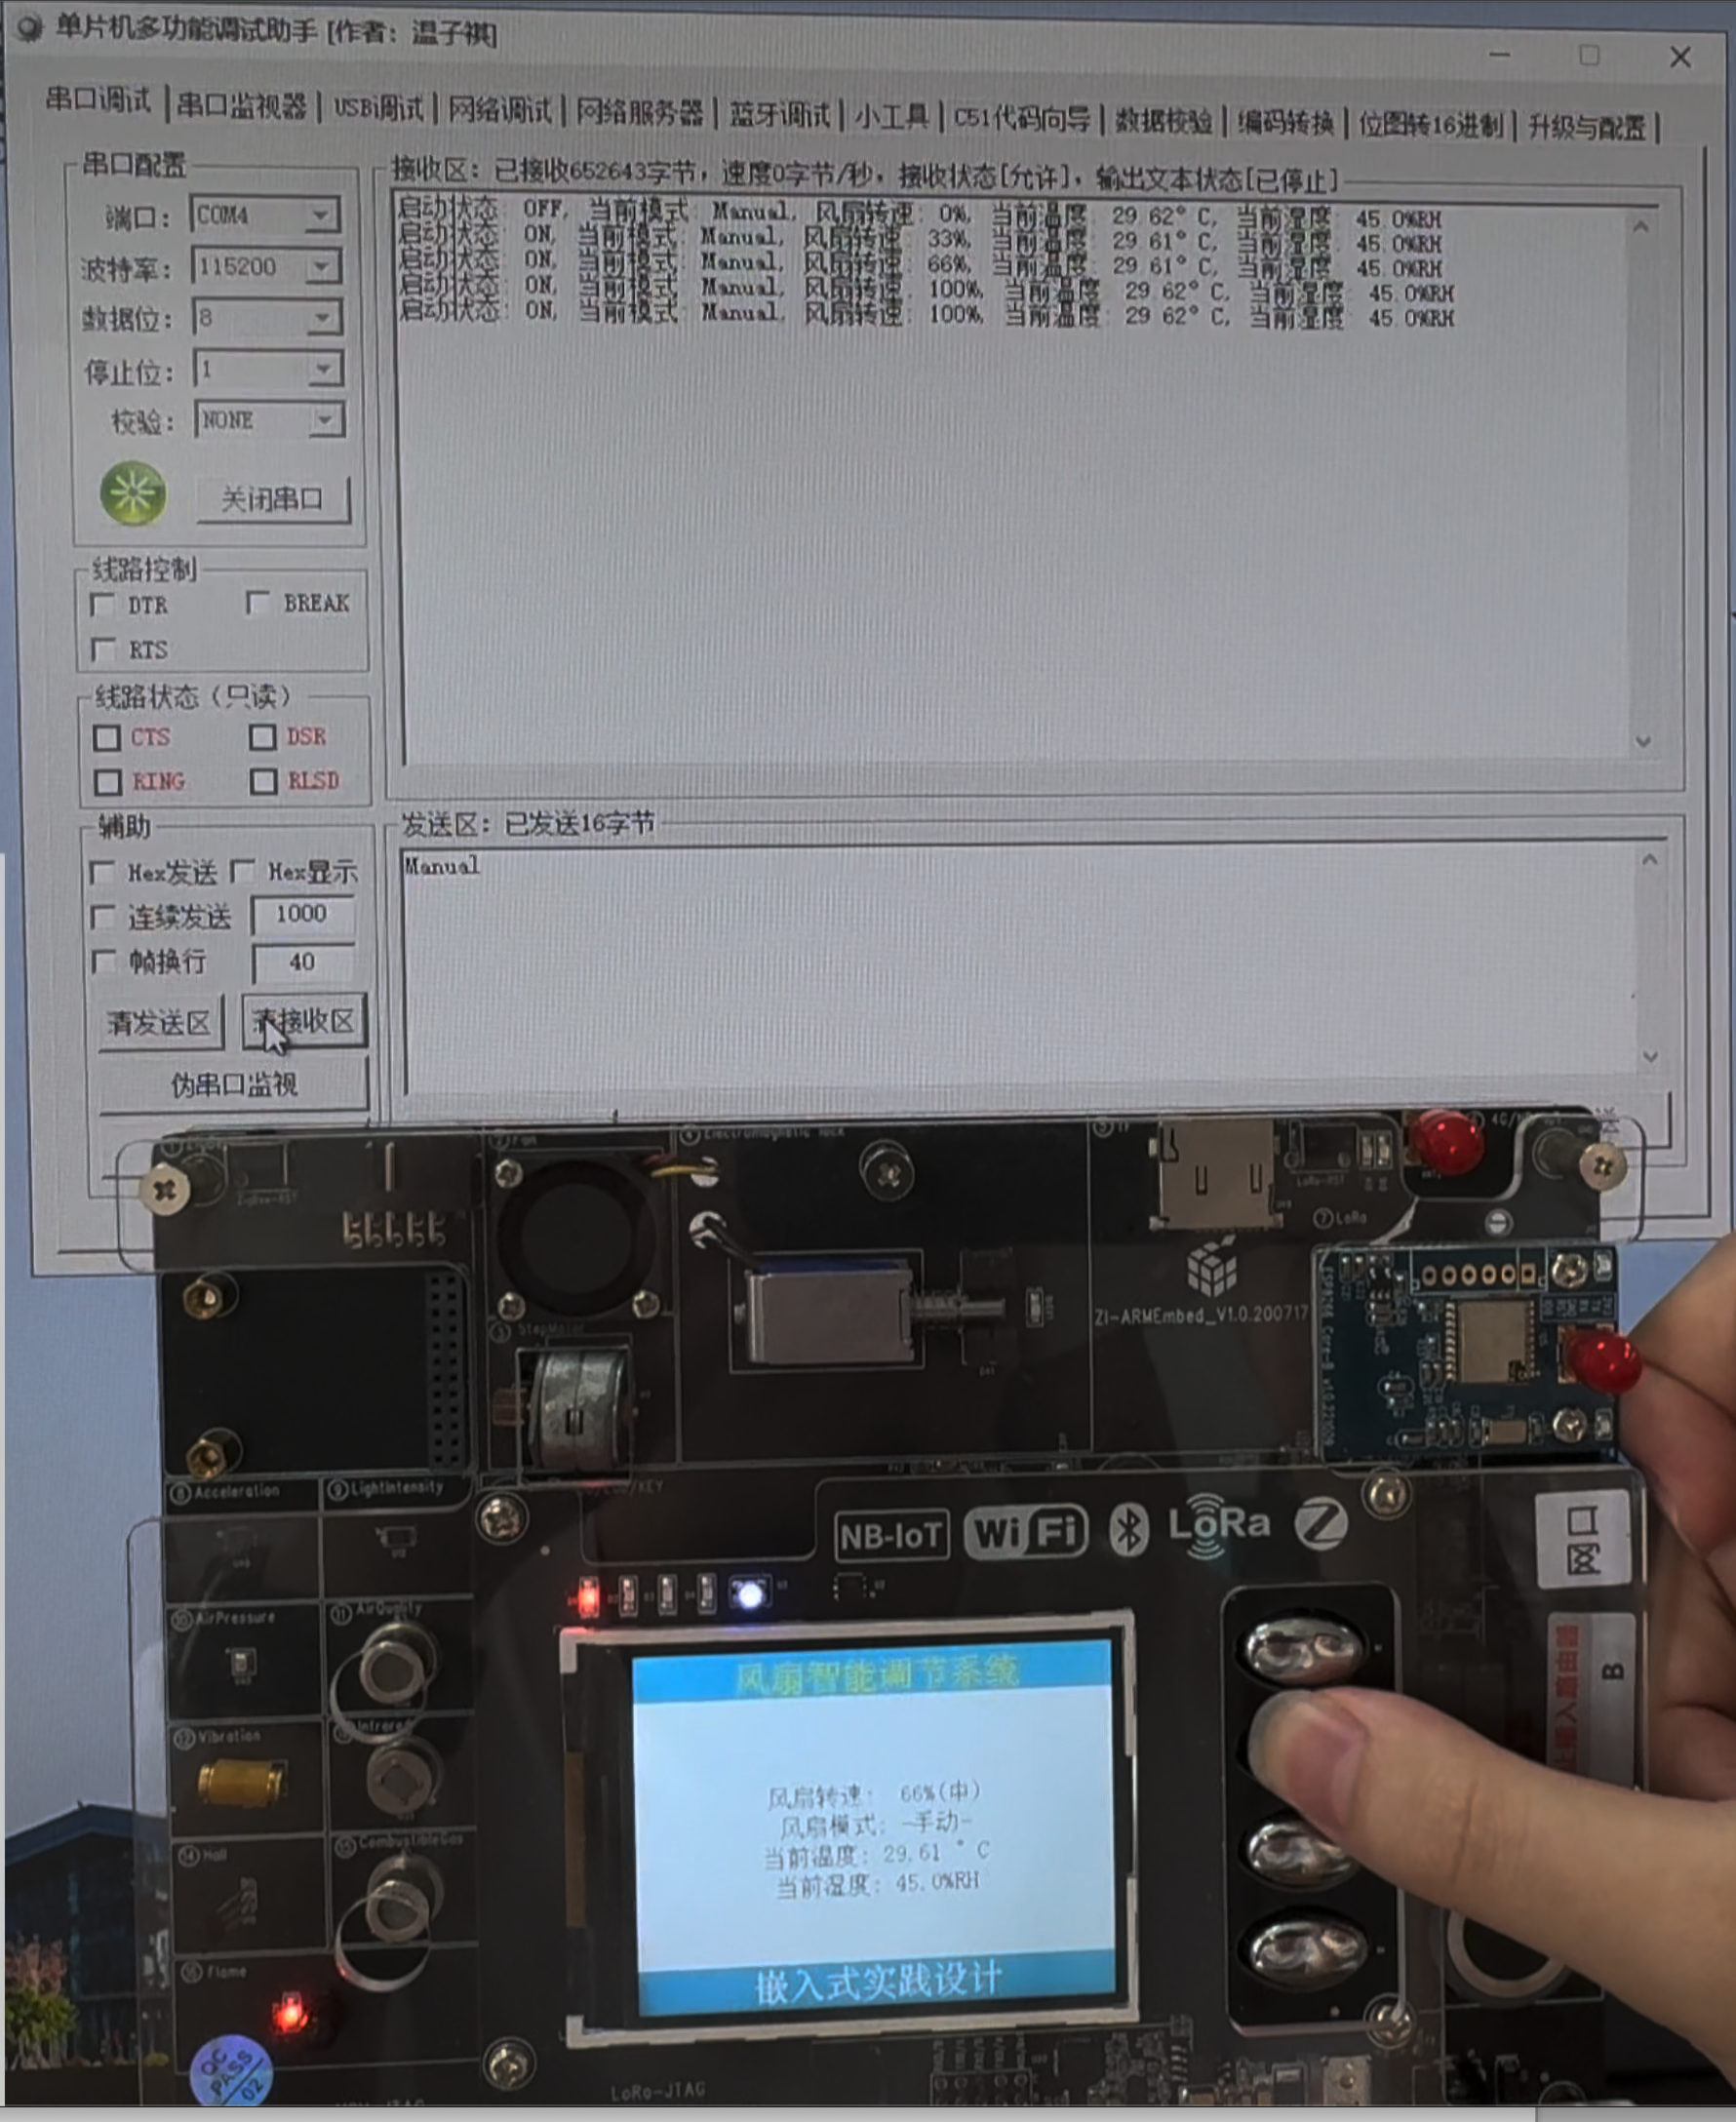
\includegraphics[width=\textwidth]{../figures/CleanShot 2025-06-11 at 11.52.44@2x.png}
    \caption{风扇转速66\%状态}
  \end{subfigure}
  \hfill
  \begin{subfigure}{0.45\textwidth}
    \centering
    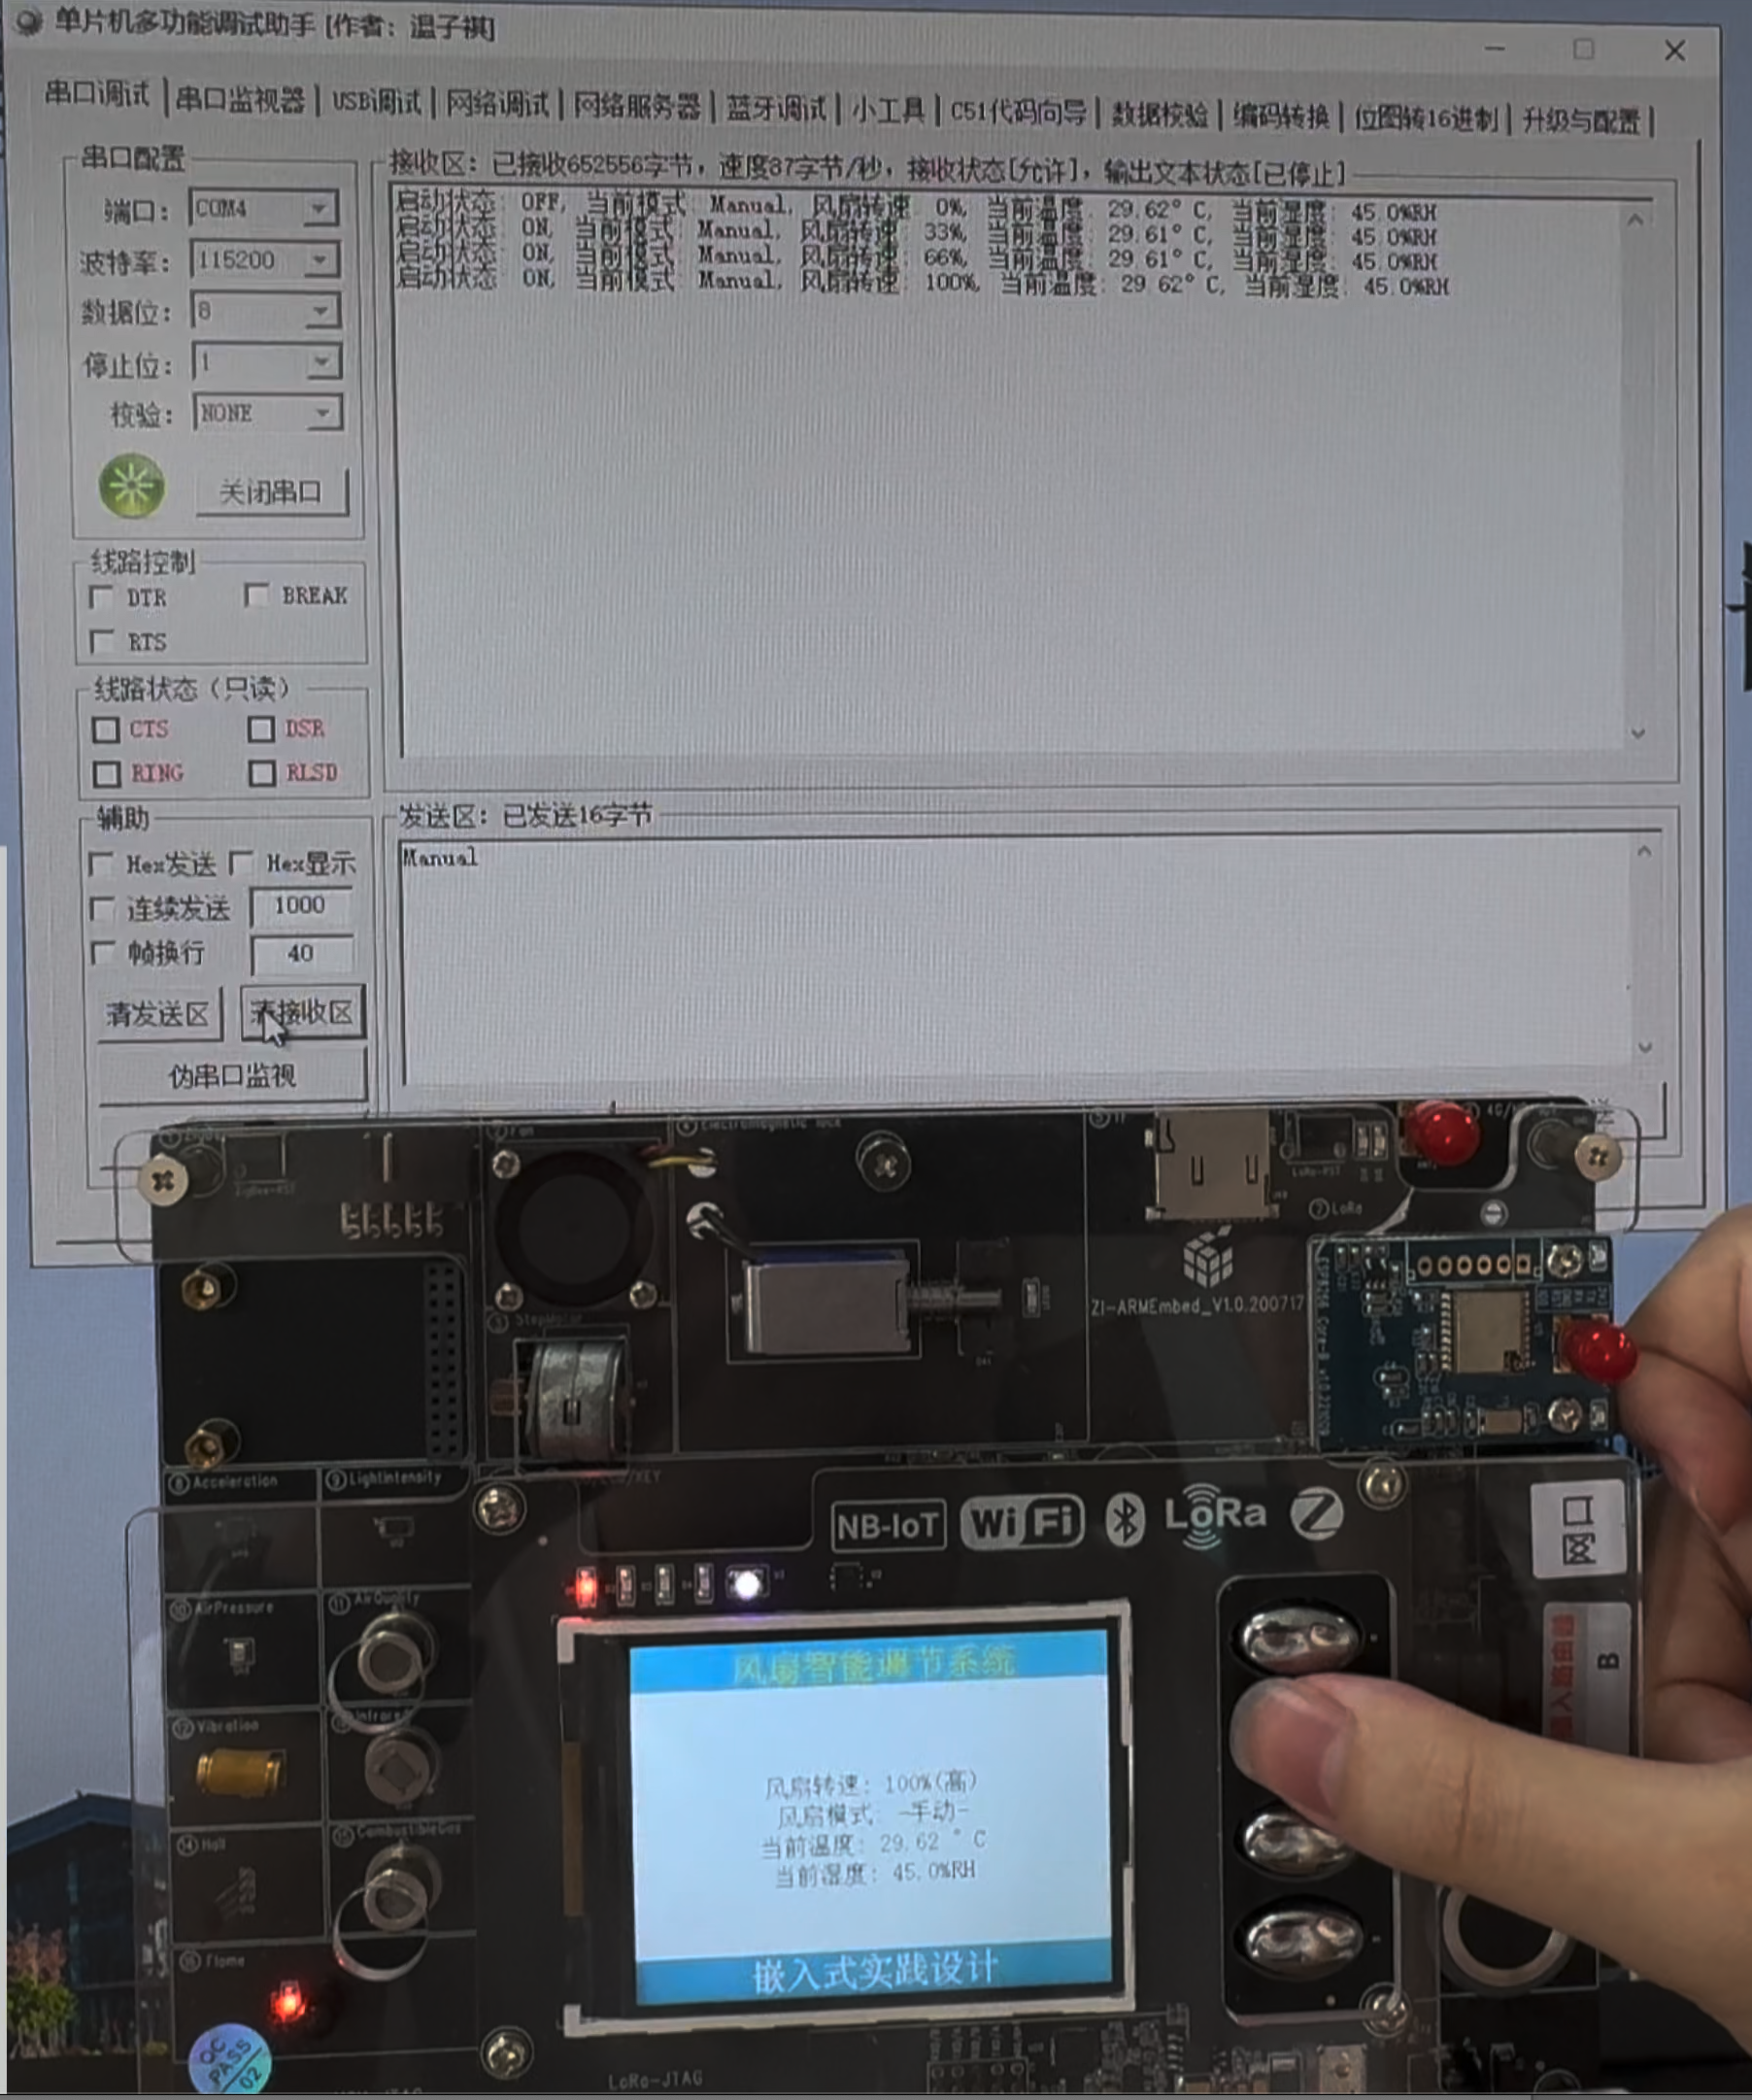
\includegraphics[width=\textwidth]{../figures/CleanShot 2025-06-11 at 11.52.25@2x.png}
    \caption{风扇转速100\%状态}
  \end{subfigure}

  \caption{RGB LED状态指示功能调试效果}
  \label{fig:rgb_led_debug}
\end{figure}

\subsubsection{蜂鸣器功能调试}

\qquad 蜂鸣器提供声音反馈,包括按键确认和高温报警等功能。

\textbf{调试内容:}
\begin{itemize}
    \vspace{-6pt}
  \item 测试蜂鸣器的基本发声功能
    \vspace{-6pt}
  \item 验证按键操作时的确认提示音
    \vspace{-6pt}
  \item 检查高温报警时的蜂鸣器响应(最多3次)
    \vspace{-6pt}
  \item 确认声音大小和持续时间的合理性
\end{itemize}

\textbf{调试方法:}通过按键操作和温度模拟测试蜂鸣器响应,验证报警机制的有效性。

\subsubsection{UART串口通信功能调试}

\qquad 串口通信实现远程控制和状态监测,是系统扩展性的重要保障。

\textbf{调试内容:}
\begin{itemize}
    \vspace{-6pt}
  \item 验证串口初始化配置(115200bps波特率)
    \vspace{-6pt}
  \item 测试"Auto"和"Manual"模式切换命令接收
    \vspace{-6pt}
  \item 检查系统状态信息的定时发送(每3ms)
    \vspace{-6pt}
  \item 确认数据传输的准确性和稳定性
\end{itemize}

\textbf{调试方法:}使用串口调试工具发送控制命令,监控系统状态输出,验证通信协议的正确性。

% 预留图片位置
\begin{figure}[H]
  \centering
  \begin{subfigure}{0.45\textwidth}
    \centering
    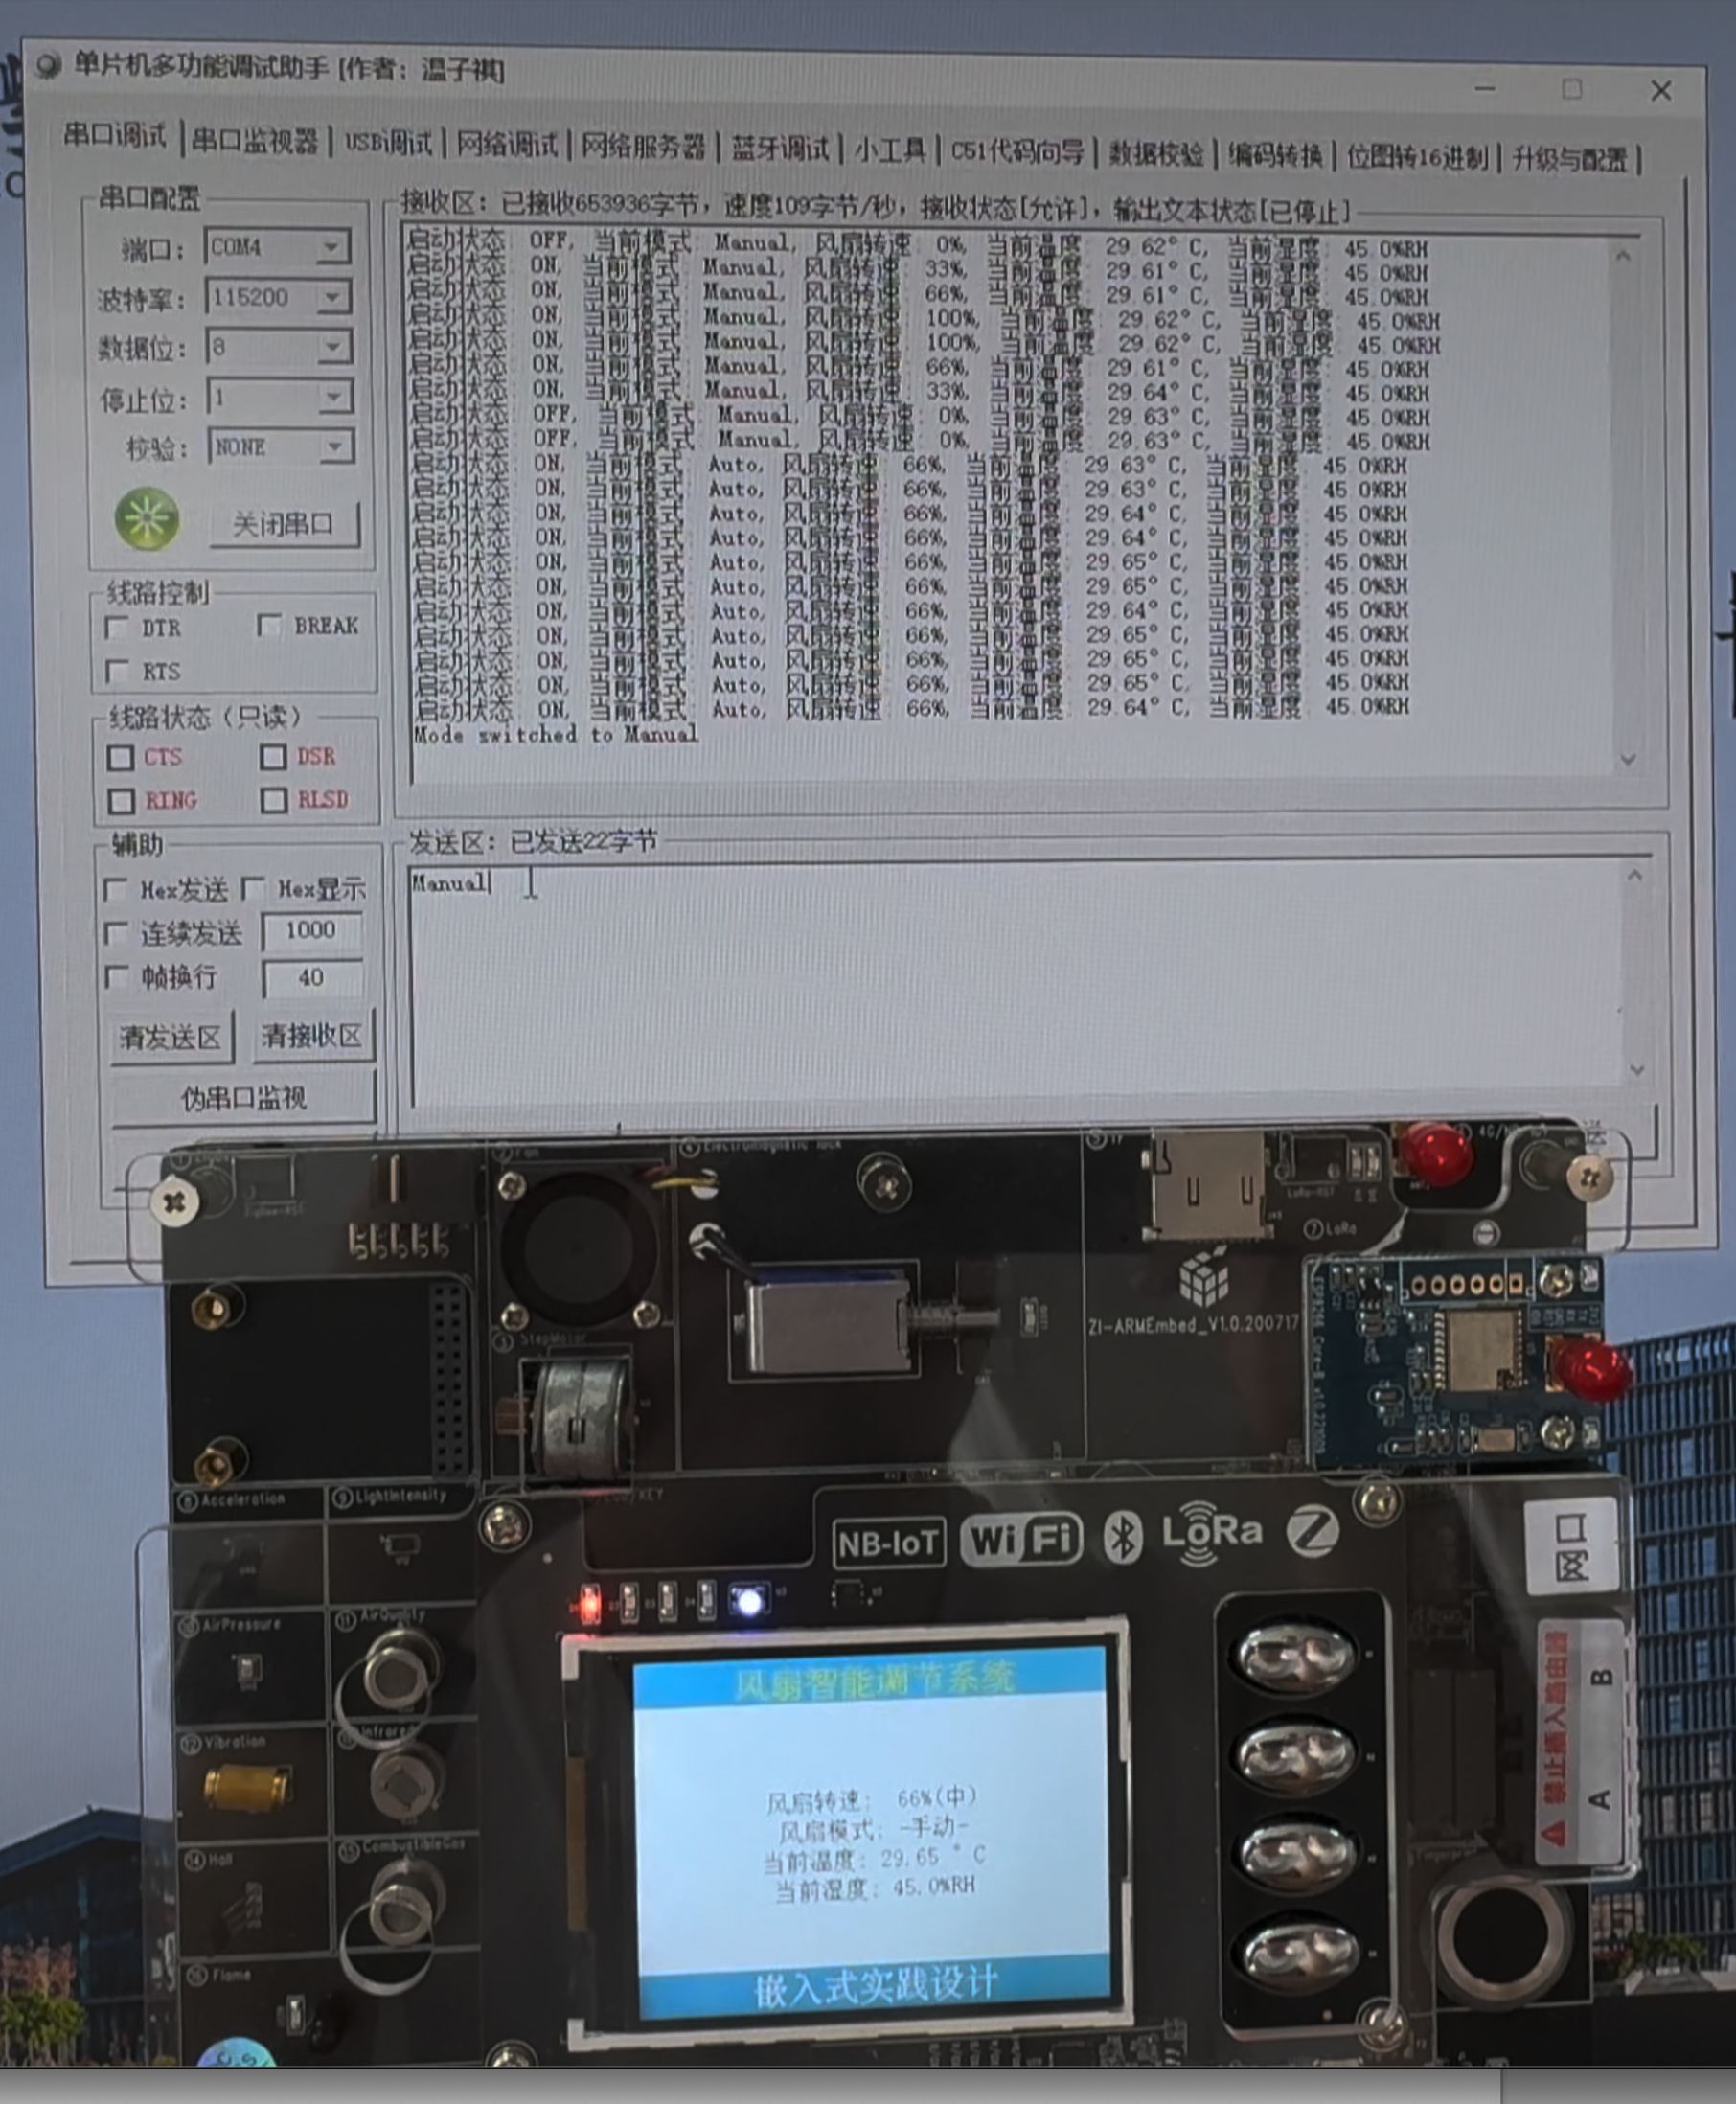
\includegraphics[width=\textwidth]{../figures/CleanShot 2025-06-11 at 12.03.40@2x.png}
    \caption{串口发送Manual状态}
  \end{subfigure}
  \hfil
  \begin{subfigure}{0.45\textwidth}
    \centering
    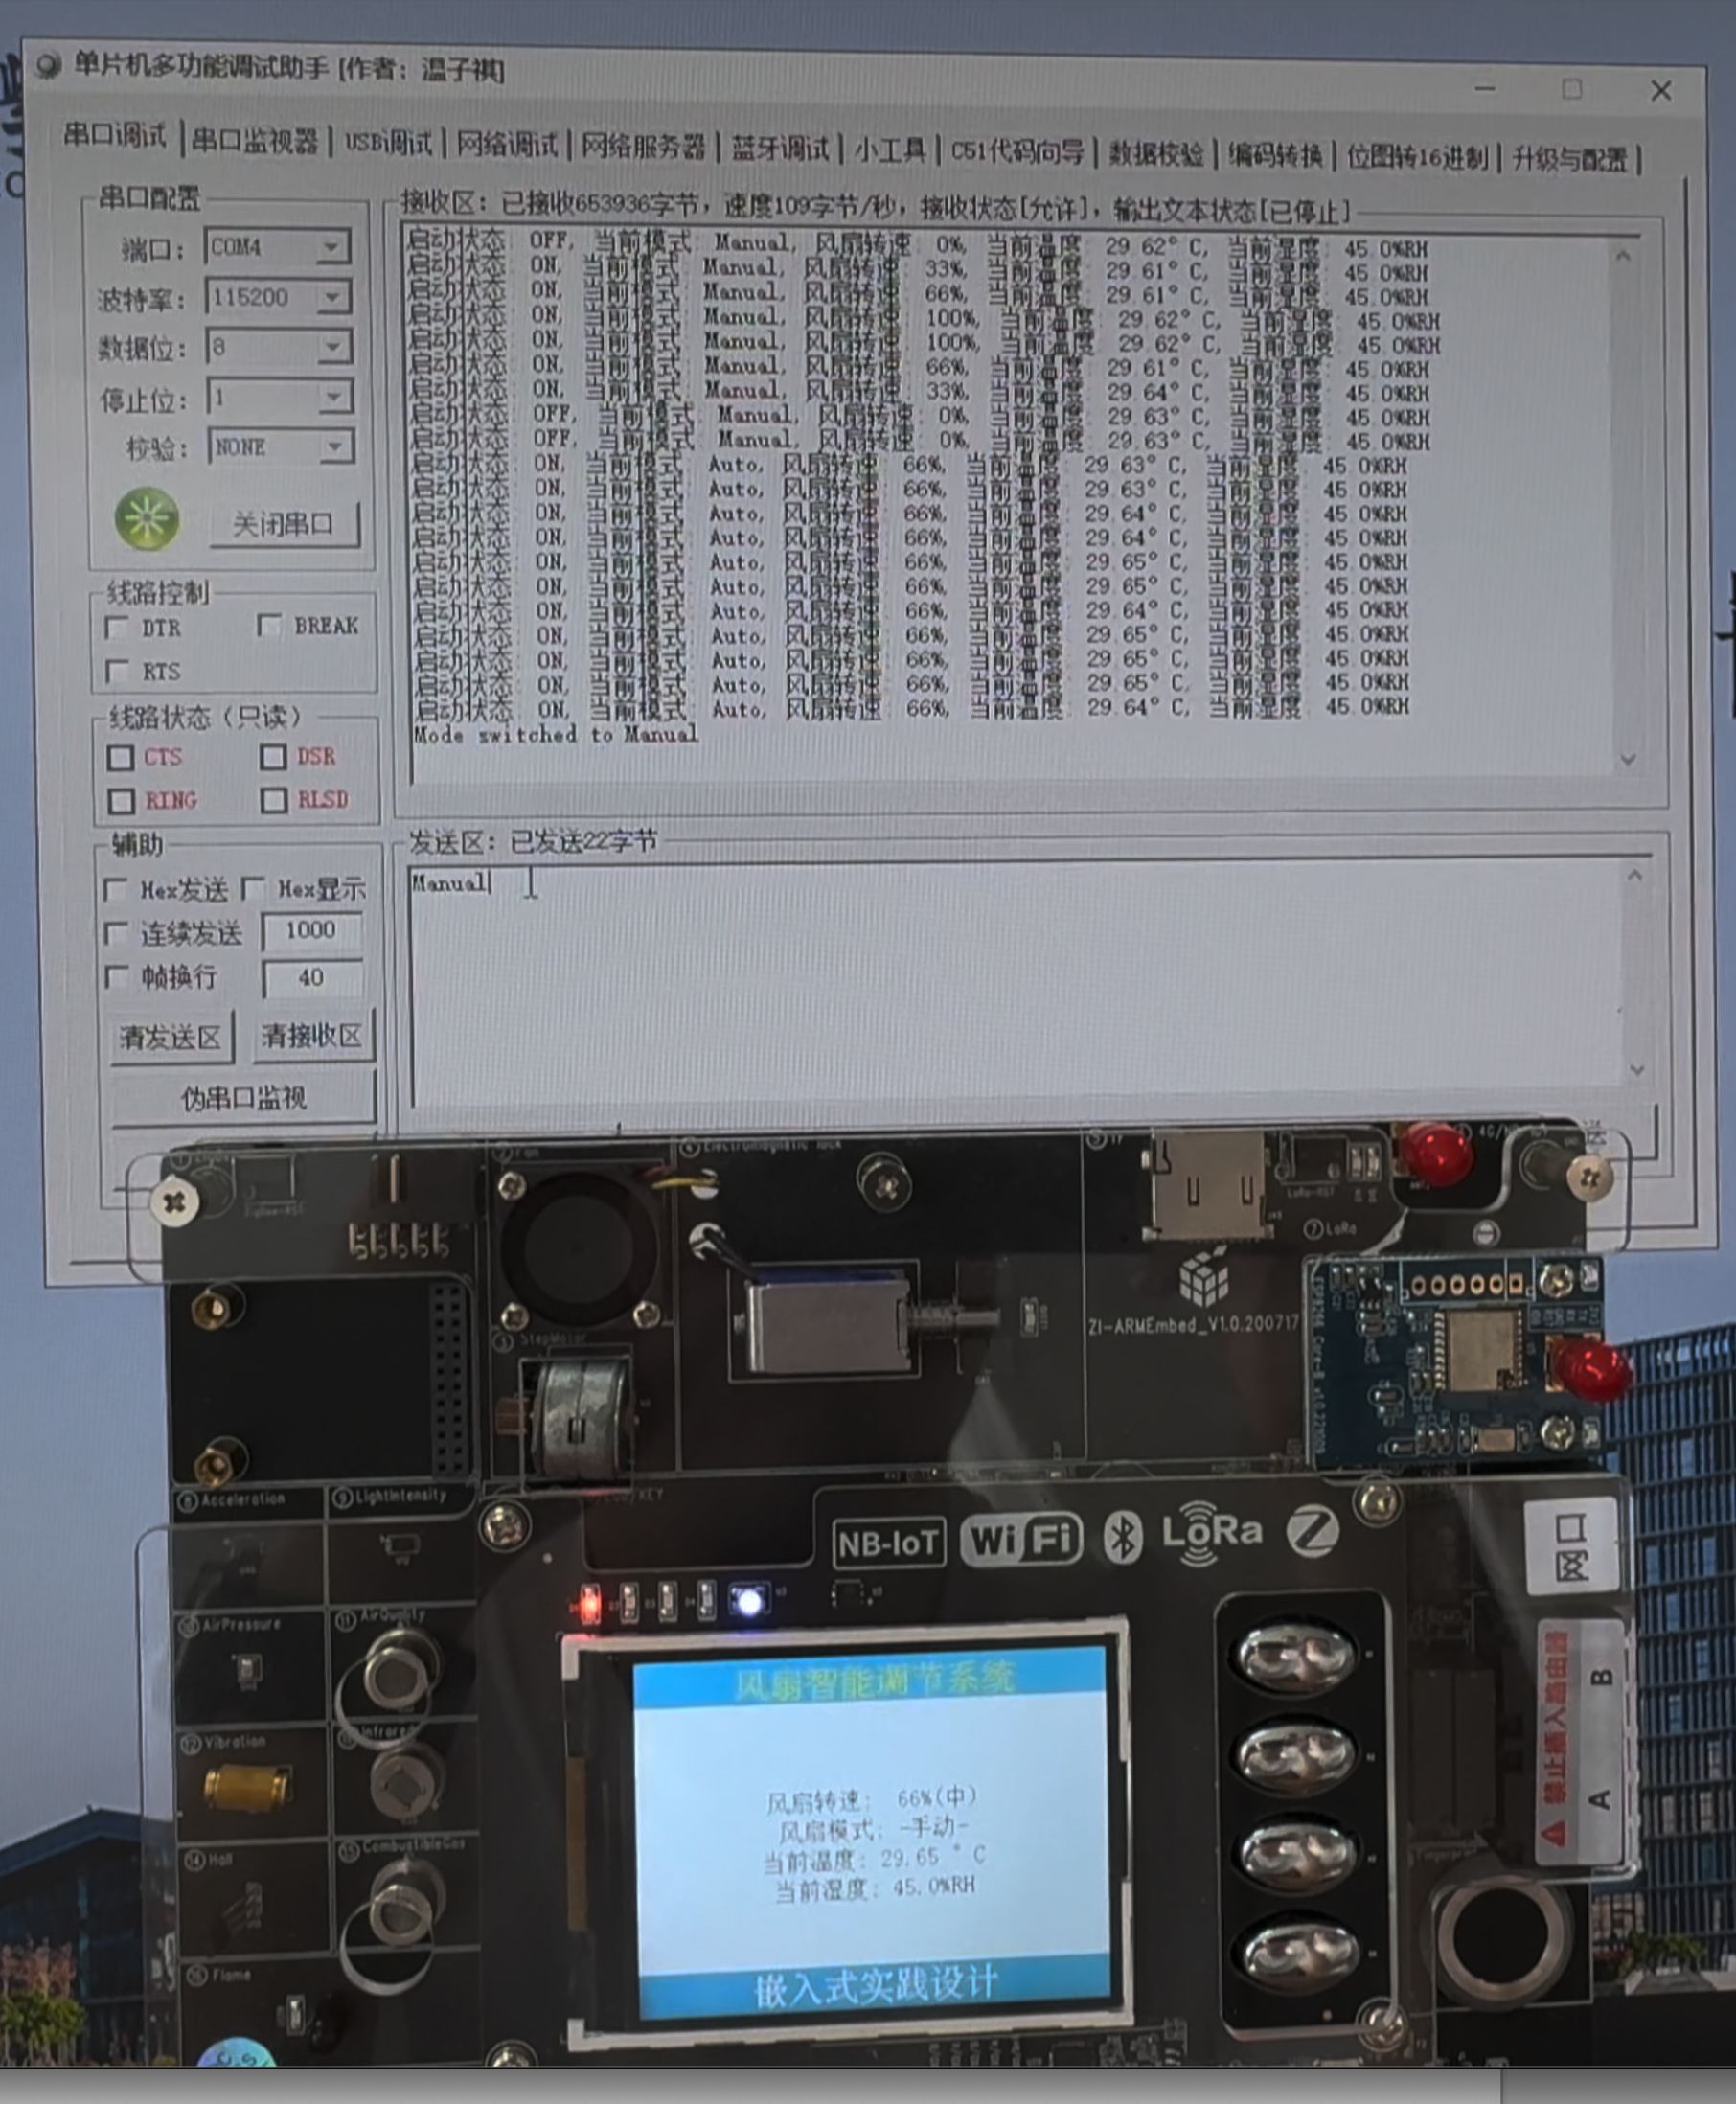
\includegraphics[width=\textwidth]{../figures/CleanShot 2025-06-11 at 12.03.40@2x.png}
    \caption{串口发送Auto状态}
  \end{subfigure}

  \caption{UART串口通信功能调试界面}
  \label{fig:uart_debug}
\end{figure}

\subsubsection{自动控制功能调试}

\qquad 自动控制是系统智能化的核心功能,需要验证温度阈值判断、自动档位调节等逻辑。

\textbf{调试内容:}
\begin{itemize}
    \vspace{-6pt}
  \item 测试温度阈值判断逻辑(20°C、25°C、30°C)
    \vspace{-6pt}
  \item 验证不同温度区间的自动档位切换
    \vspace{-6pt}
  \item 检查高温报警机制的触发条件
    \vspace{-6pt}
  \item 确认自动控制的响应速度和准确性
\end{itemize}

\textbf{调试方法:}通过温度模拟或环境温度变化测试自动控制逻辑,观察档位切换和状态指示。

% 预留图片位置
\begin{figure}[H]
  \centering
  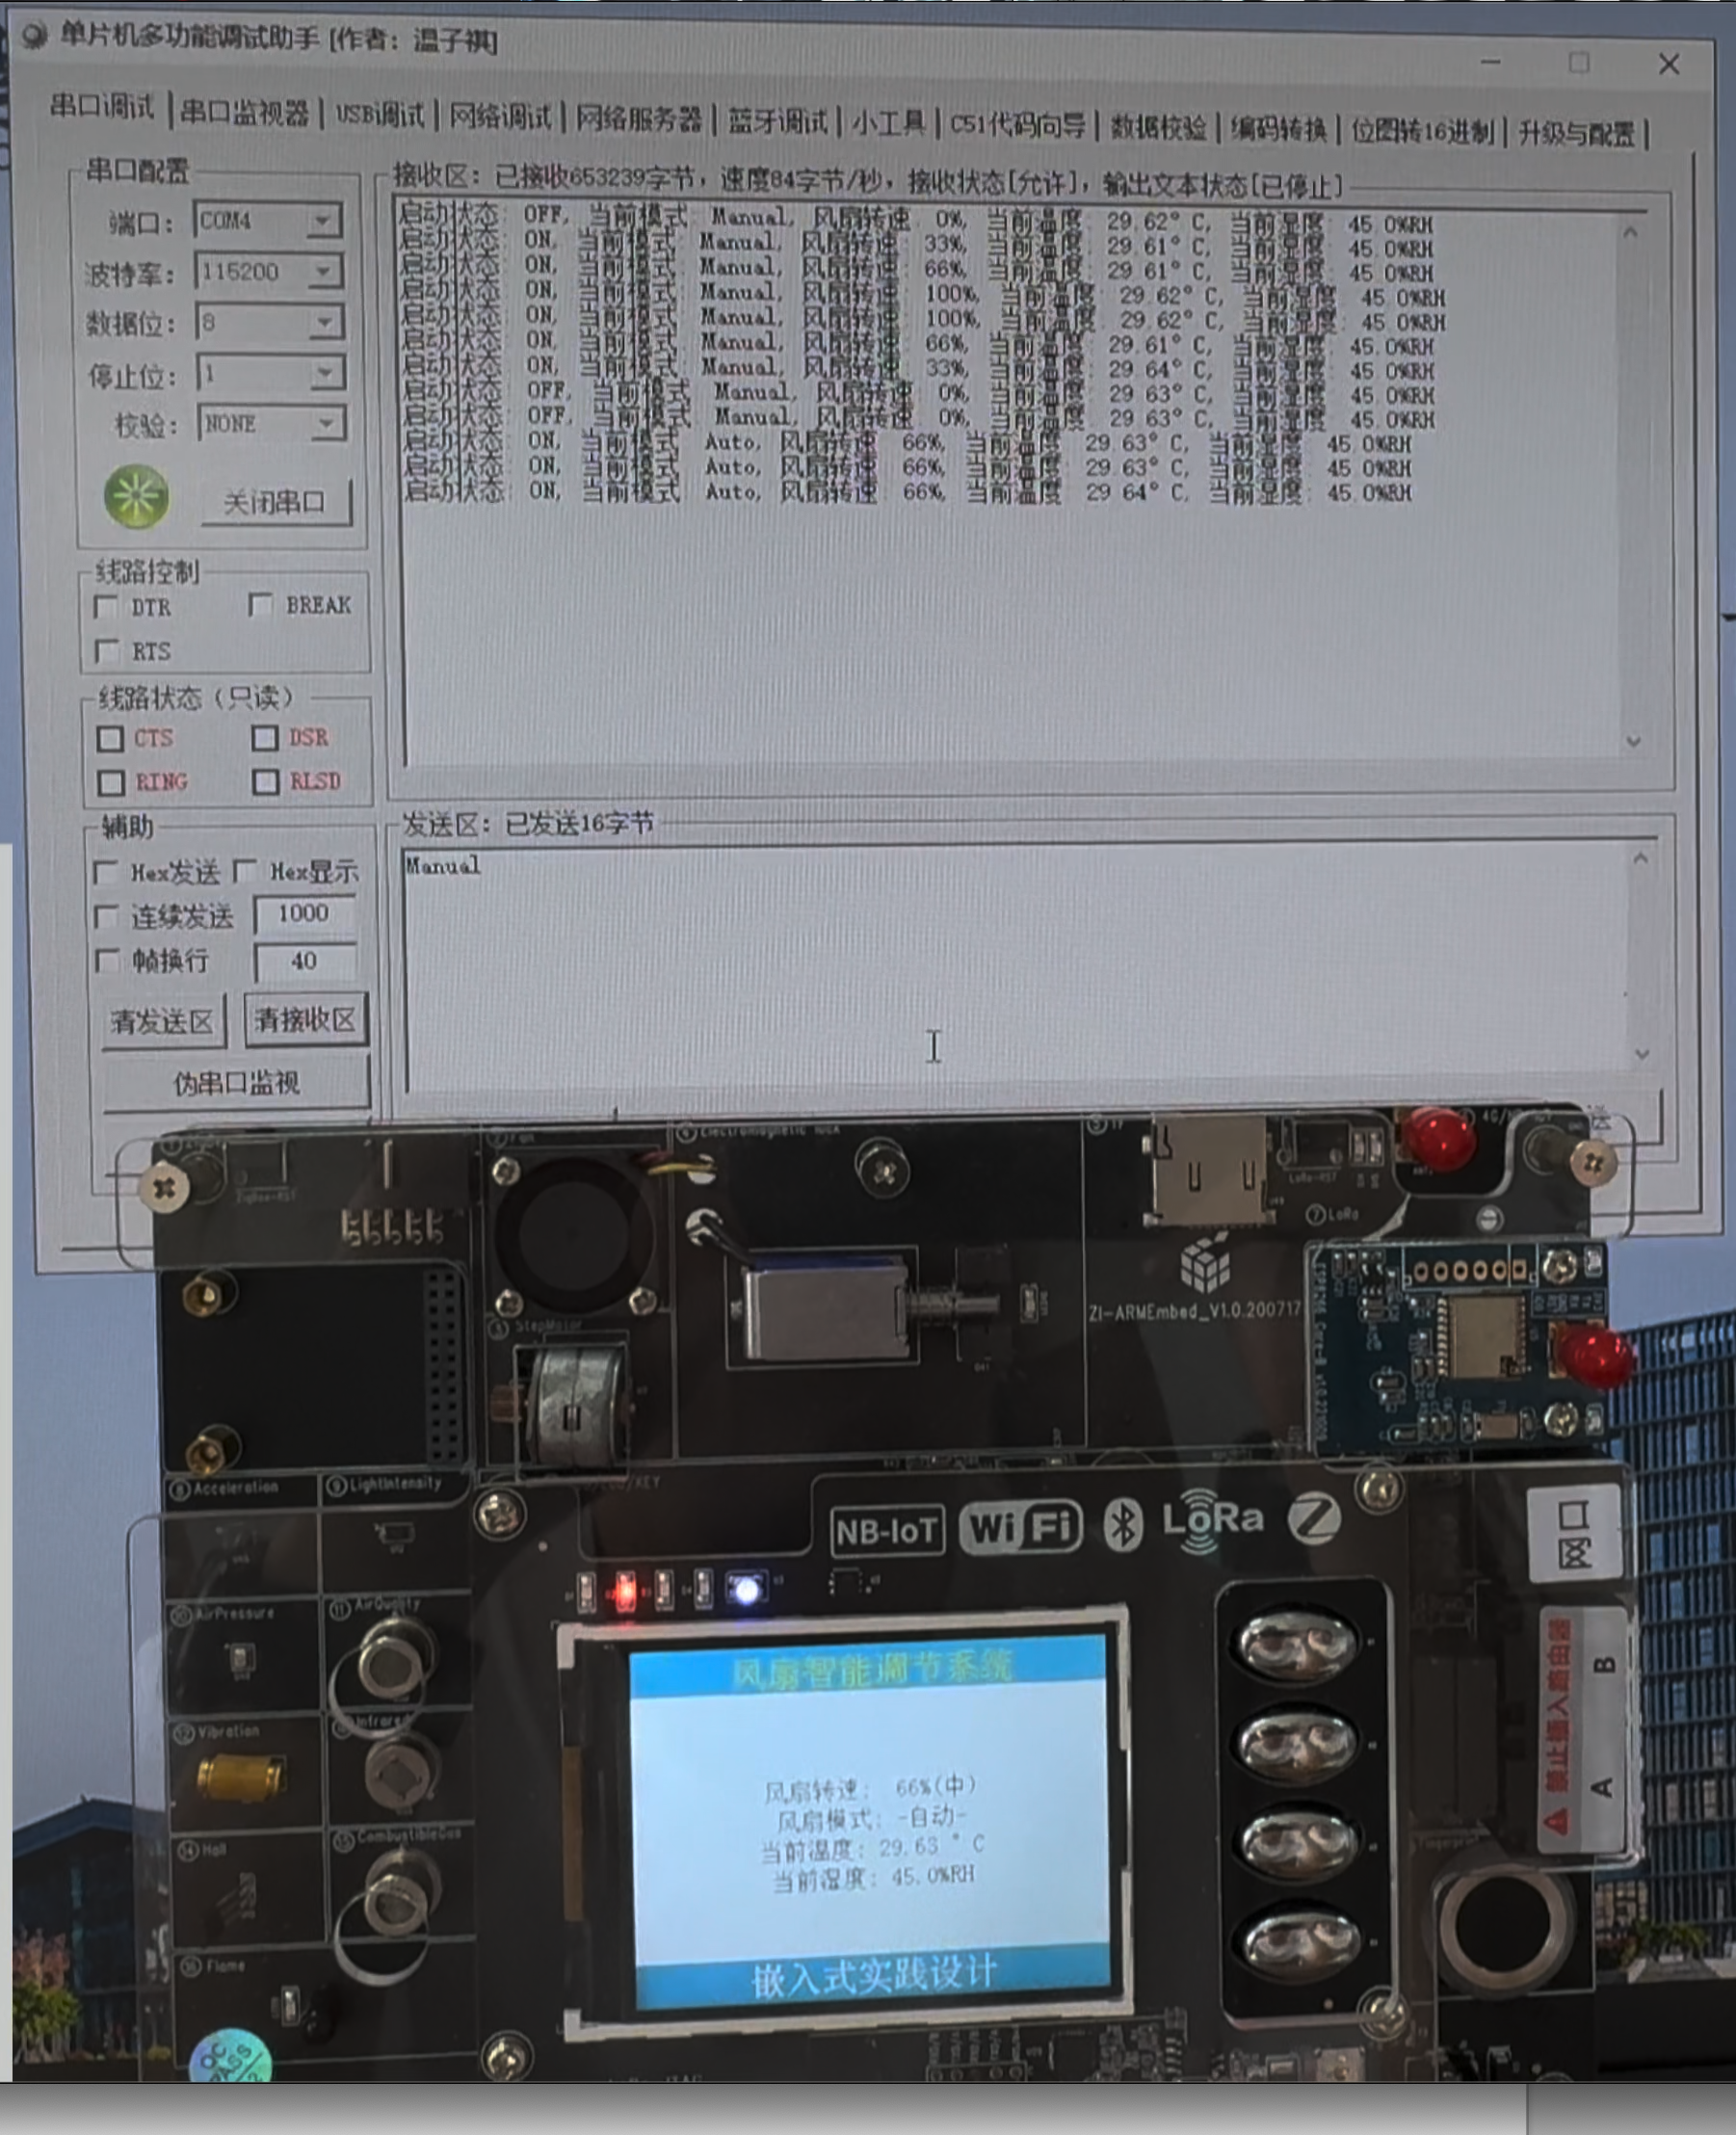
\includegraphics[width=0.45\textwidth]{../figures/CleanShot 2025-06-11 at 12.05.56@2x.png}
  \caption{自动控制功能调试过程}
  \label{fig:auto_control_debug}
\end{figure}

\subsubsection{手动控制功能调试}

\qquad 手动控制提供用户自主操作能力,需要验证按键响应、档位调节等功能。

\textbf{调试内容:}
\begin{itemize}
    \vspace{-6pt}
  \item 测试K1按键增加档位功能
    \vspace{-6pt}
  \item 验证K2按键减少档位功能
    \vspace{-6pt}
  \item 检查档位边界保护机制(0-3档)
    \vspace{-6pt}
  \item 确认手动模式下的状态指示正确性
\end{itemize}

\textbf{调试方法:}在手动模式下测试档位调节,验证边界条件处理和用户体验。

\subsubsection{系统开关功能调试}

\qquad 系统开关功能是基本的电源管理功能,需要验证状态切换、数据保持等。

\textbf{调试内容:}
\begin{itemize}
    \vspace{-6pt}
  \item 测试K4按键的系统开关功能
    \vspace{-6pt}
  \item 验证关机状态下的风扇停止运行
    \vspace{-6pt}
  \item 检查开机状态的功能恢复
    \vspace{-6pt}
  \item 确认状态监测功能在关机状态下的保持
\end{itemize}

\textbf{调试方法:}反复测试开关机功能,验证状态保存和恢复的正确性。
